\documentclass[12pt, a4paper]{article}

% --- Packages ---
\usepackage[utf8]{inputenc}
\usepackage[T1]{fontenc}
\usepackage[french]{babel}
\usepackage{graphicx}
\usepackage{booktabs}
\usepackage{amsmath}
\usepackage{geometry}
\usepackage{array}
\usepackage{enumitem}
\usepackage{hyperref}
\usepackage{xcolor}
\usepackage{titlesec}

\usepackage{lmodern}
\usepackage{microtype}
\usepackage{fancyhdr}

% --- Font Configuration ---


% --- Color Definitions ---
\definecolor{primary}{RGB}{0,51,102}
\definecolor{secondary}{RGB}{102,102,153}
\definecolor{accent}{RGB}{204,0,0}

% --- Page Geometry ---
\geometry{
  a4paper,
  left=2.5cm,
  right=2.5cm,
  top=2.5cm,
  bottom=2.5cm,
  headheight=15pt
}

% --- Header/Footer Setup ---
\pagestyle{fancy}
\fancyhf{}
\fancyhead[L]{\small Rapport de Stage - Semaine 1}
\fancyhead[R]{\small Zakaria el Khaldi}
\fancyfoot[C]{\thepage}
\renewcommand{\headrulewidth}{0.4pt}
\renewcommand{\footrulewidth}{0.4pt}

% --- Title Formatting ---
\titleformat{\section}
  {\normalfont\Large\bfseries\color{primary}}
  {\thesection}{1em}{}
\titleformat{\subsection}
  {\normalfont\large\bfseries\color{secondary}}
  {\thesubsection}{1em}{}
\titleformat{\subsubsection}
  {\normalfont\normalsize\bfseries\color{accent}}
  {\thesubsubsection}{1em}{}

% --- List Formatting ---
\setlist[itemize]{leftmargin=*, nosep}
\setlist[enumerate]{leftmargin=*, nosep}

% --- Hyperlink Setup ---
\hypersetup{
  colorlinks=true,
  linkcolor=primary,
  urlcolor=secondary,
  citecolor=accent
}

% --- Title Page Information ---
\title{\Huge\bfseries\color{primary} Rapport de Stage \\ 
      \Large Semaine 1 : Conception et Architecture d'une Plateforme E-learning}
\author{\Large Zakaria el Khaldi}
\date{\large Le 10 mai 2025}

% --- Document Start ---
\begin{document}

% --- Cover Page ---
\begin{titlepage}
  \centering
  \vspace*{\stretch{0.5}}
  {\Huge\bfseries\color{primary} Rapport de Stage \par}
  \vspace{1cm}
  {\Large\itshape Semaine 1 : Conception et Architecture d'une Plateforme E-learning\par}
  \vspace{2cm}
  
  \vspace{2cm}
  {\Large Zakaria el Khaldi\par}
  \vfill
  {\large Le 10 mai 2025\par}
  \vspace*{\stretch{1}}
\end{titlepage}

% --- Table of Contents ---
\tableofcontents
\thispagestyle{empty}
\newpage

% --- Introduction ---
\section{Introduction}
\thispagestyle{fancy}
Ce rapport détaille les travaux réalisés durant la première semaine de stage. L'objectif principal de ce stage est le développement d'une plateforme e-learning complète destinée aux entreprises et aux professionnels individuels. Cette première semaine a été consacrée à la phase de conception initiale du projet, à la définition de l'architecture backend et des bases de données, ainsi qu'à la création des premiers diagrammes UML.

% --- Week 1 Accomplishments ---
\section{Bilan de la Semaine 1}

\subsection{Conception du Projet}
La phase initiale de conception s'est concentrée sur la définition de la vision, des offres, des utilisateurs cibles et de la valeur unique de la plateforme.

\subsubsection{Vision de la Plateforme}
\begin{itemize}
  \item \textbf{Idée Principale :} Une plateforme e-learning complète pour les entreprises et les professionnels individuels.
  \item \textbf{Offres Clés :}
    \begin{itemize}
      \item Cours en ligne auto-rythmés (vidéos, images, quiz)
      \item Services de support, de conseil et de « prestation » via une plateforme de réunion personnalisée intégrée
    \end{itemize}
  \item \textbf{Utilisateurs Cibles :} Entreprises (pour la formation des employés) et apprenants individuels (pour l'amélioration des compétences)
  \item \textbf{Valeur Unique :} Un mélange harmonieux d'apprentissage structuré et d'interaction avec des experts à la demande
\end{itemize}

\subsubsection{Acteurs Utilisateurs Clés}
Les principaux types d'utilisateurs identifiés pour la plateforme sont :
\begin{itemize}
  \item \textbf{Apprenant Individuel :} S'inscrit, s'abonne, apprend, demande des consultations
  \item \textbf{Employé d'Entreprise :} Apprend via l'abonnement de l'entreprise, demande des consultations
  \item \textbf{Administrateur/Manager d'Entreprise :} Gère le compte de l'entreprise, les employés, les abonnements, attribue les cours, consulte les analyses
  \item \textbf{Créateur de Cours :} Conçoit et élabore le contenu des cours (modules, leçons, quiz)
  \item \textbf{Consultant/Fournisseur de Prestations :} Gère sa disponibilité, anime les sessions via la plateforme de réunion
  \item \textbf{Agent de Support Plateforme :} Assiste les utilisateurs pour les problèmes liés à la plateforme et les questions-réponses
  \item \textbf{Administrateur de la Plateforme :} Supervise l'ensemble de la plateforme, les utilisateurs, le contenu, les paramètres
\end{itemize}

\subsubsection{Fonctionnalités Principales de la Plateforme}
Les fonctionnalités essentielles se divisent en trois catégories :
\begin{itemize}
    \item \textbf{E-Learning :}
    \begin{itemize}
        \item Catalogue de cours (filtrable, consultable)
        \item Modules, Leçons (vidéo, basées sur des images)
        \item Quiz et Évaluations
        \item Suivi de la Progression
        \item Certificats de Réussite
        \item Support Multilingue (EN/FR)
        \item Paramètres Utilisateur et Entreprise
    \end{itemize}
    \item \textbf{Consultation et Prestation :}
    \begin{itemize}
        \item Navigation des services
        \item Profils des consultants et disponibilité
        \item Système de réservation/demande
        \item Intégration API avec la plateforme de réunion personnalisée
        \item Facturation des sessions (via la plateforme de réunion)
    \end{itemize}
    \item \textbf{Monétisation :}
    \begin{itemize}
        \item Abonnements pour utilisateurs individuels (accès illimité)
        \item Abonnements pour entreprises (par utilisateur)
        \item Réductions et Démos
    \end{itemize}
\end{itemize}

\subsection{Diagrammes UML}
\begin{figure}[h!]
  \centering
  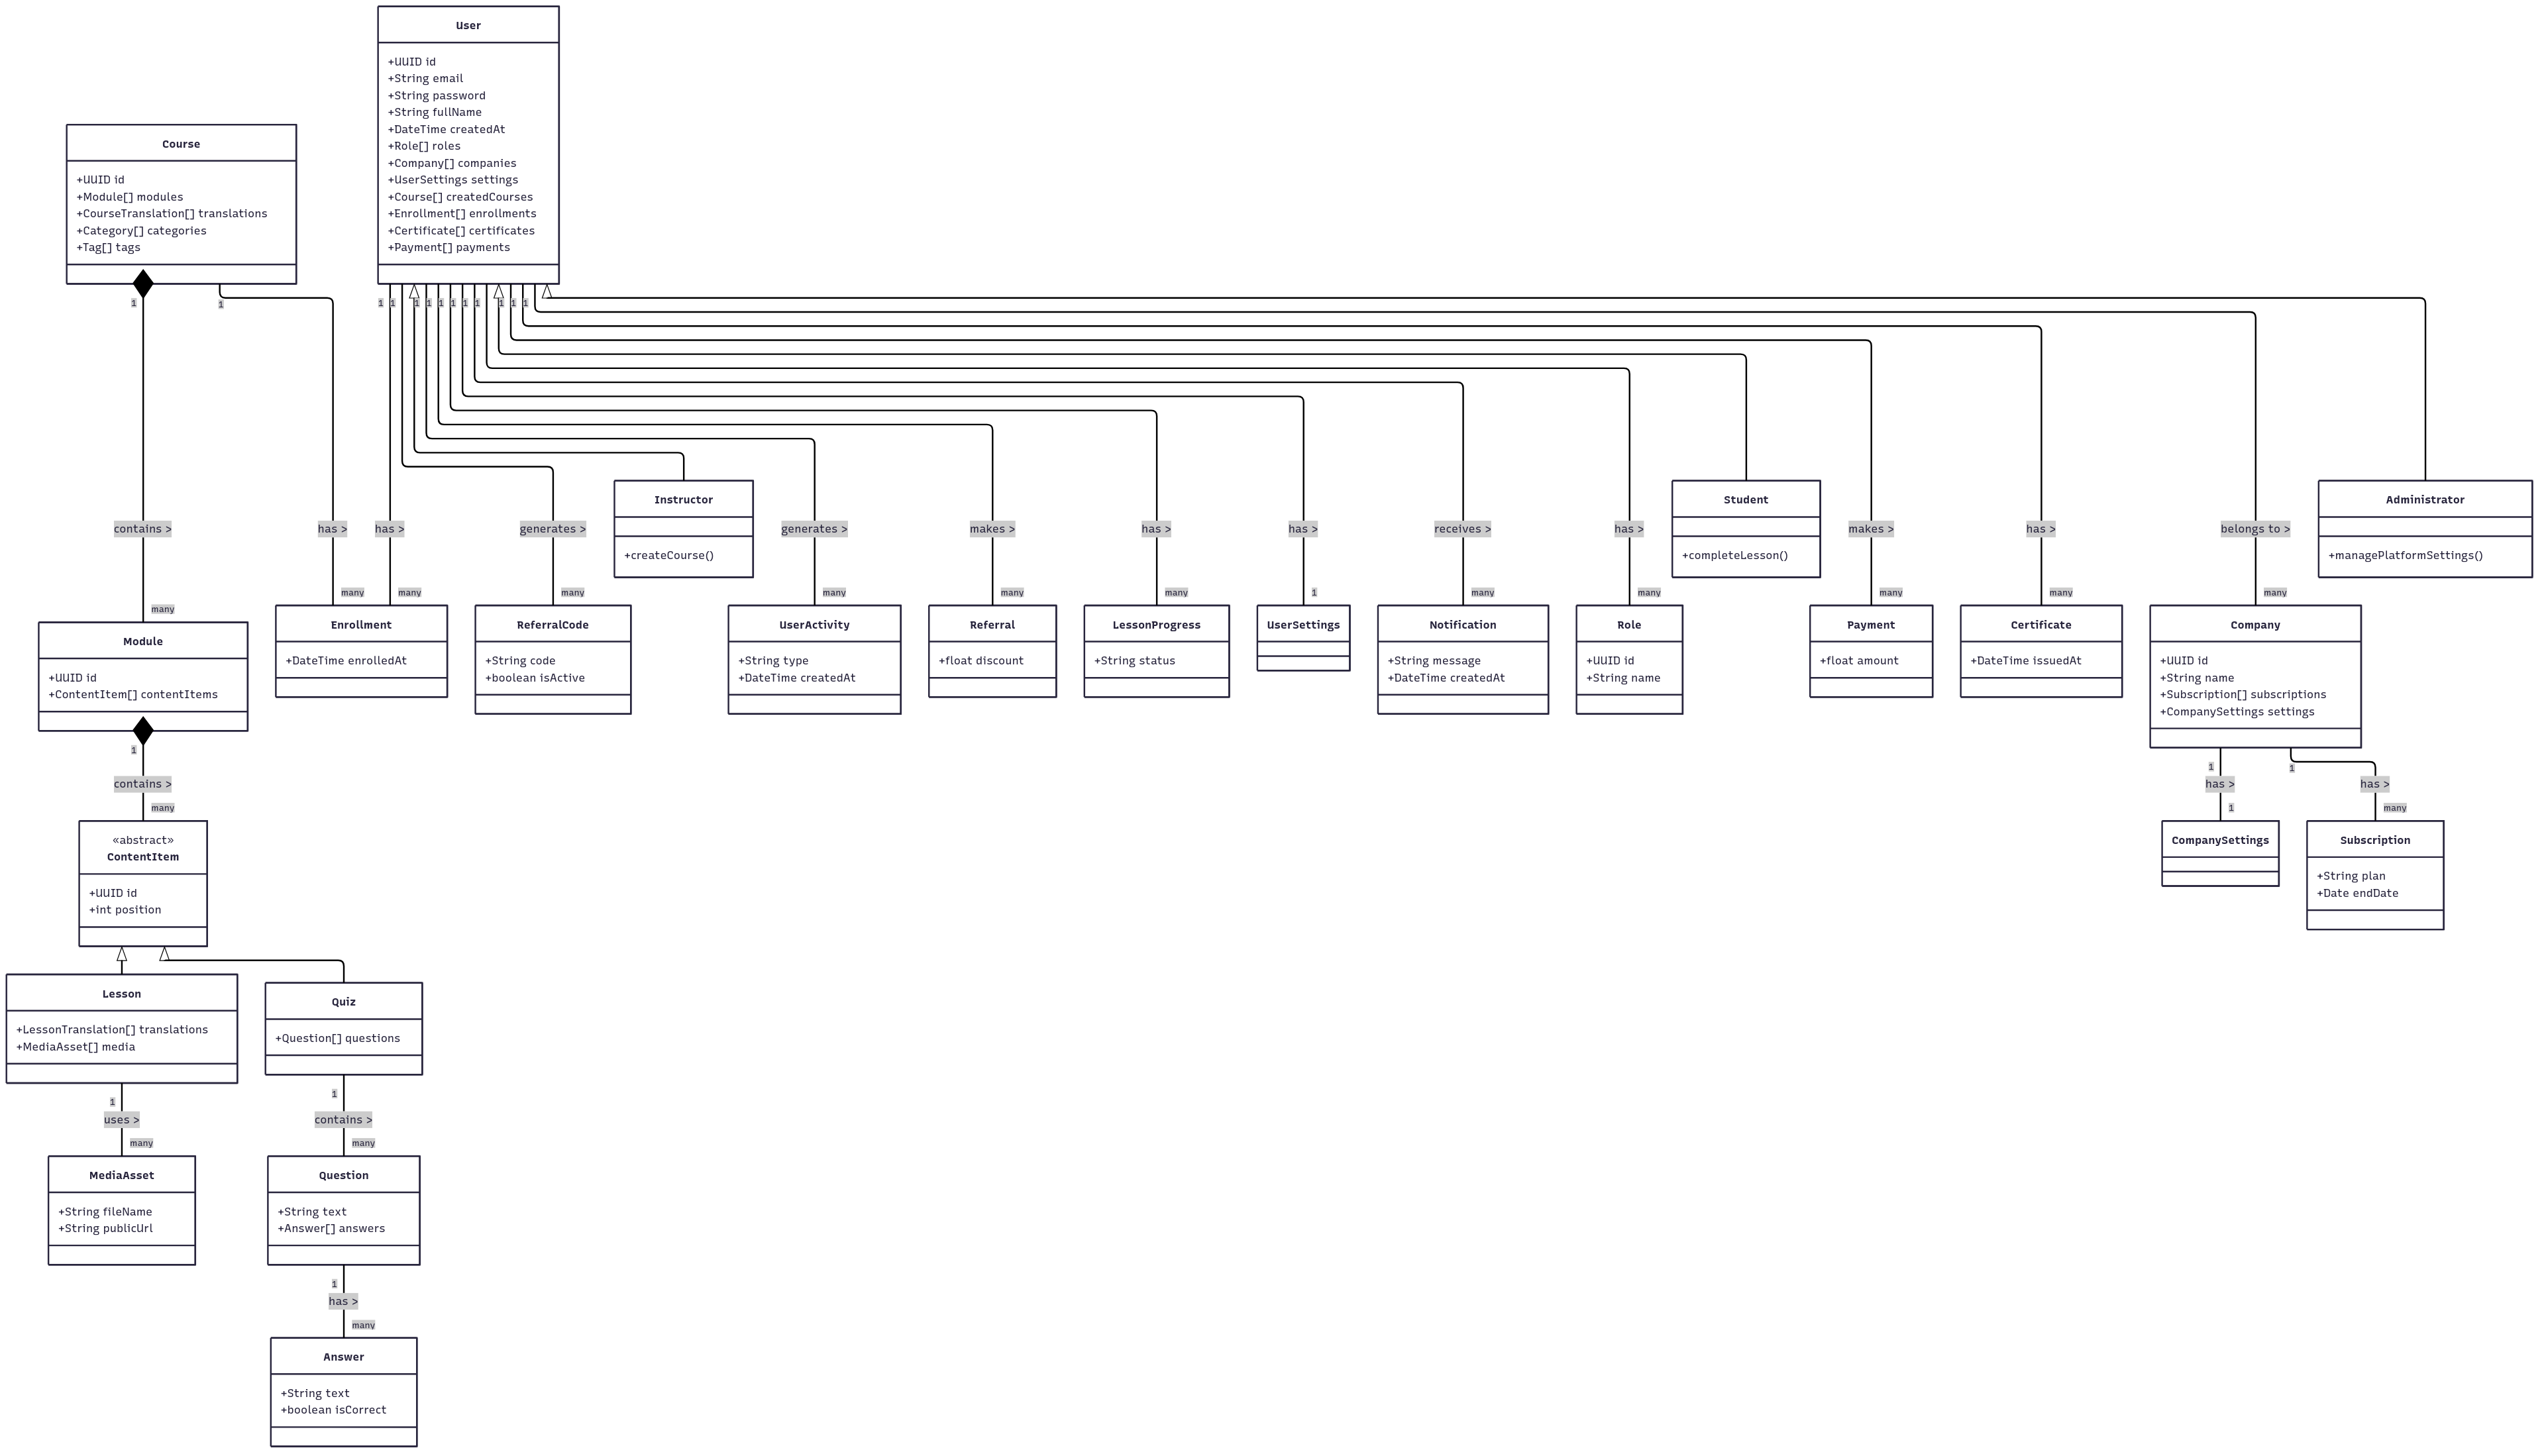
\includegraphics[width=0.9\textwidth,keepaspectratio]{class_diagrame.png}
  \caption{\textbf{Diagramme de classes initial} de la plateforme e-learning.}
  \label{fig:class_diagram}
\end{figure}

\subsection{Architecture Backend et Base de Données}
L'architecture envisagée pour la plateforme repose sur une approche de microservices.

\subsubsection{Justification des Microservices}
Le choix d'une architecture microservices est motivé par plusieurs avantages :
\begin{itemize}
  \item \textbf{Scalabilité :} Mettre à l'échelle les services individuels de manière indépendante
  \item \textbf{Maintenabilité :} Modifier des parties sans impacter l'ensemble du système
  \item \textbf{Résilience :} Une défaillance dans un service est moins susceptible de paralyser toute la plateforme
  \item \textbf{Autonomie des Équipes :} Différentes équipes peuvent posséder et déployer leurs services
  \item \textbf{Diversité Technologique :} Utiliser le meilleur outil pour chaque tâche (dans la mesure du raisonnable)
\end{itemize}

\subsubsection{Composants Architecturaux Clés}
\begin{itemize}
  \item Passerelle API (par exemple, Nginx)
  \item Communication Asynchrone (par exemple, Kafka)
  \item Conteneurisation (Docker)
\end{itemize}

\subsubsection{Pile Technologique Proposée}
La pile technologique envisagée pour le développement est la suivante :
\begin{itemize}
  \item \textbf{Frontend :} Next.js (React)
  \item \textbf{Microservices Backend :}
    \begin{itemize}
      \item Go (pour les services critiques en performance et concurrents comme les Notifications, le backend de la plateforme de réunion)
      \item Python avec FastAPI (pour les services gourmands en données, développement rapide d'API, par exemple, Catalogue de Cours, Facturation)
      \item Node.js avec Express (TypeScript) (pour les opérations I/O intensives, interaction Supabase, par exemple, IAM, Gestion des Médias)
    \end{itemize}
  \item \textbf{Bases de Données :}
    \begin{itemize}
      \item PostgreSQL (stockage relationnel principal pour la plupart des services)
      \item Supabase (pour l'Authentification, le Stockage, et son Postgres géré pour des services spécifiques)
    \end{itemize}
  \item \textbf{Passerelle API :} Nginx (en tant que reverse proxy et passerelle)
  \item \textbf{Broker de Messages :} Apache Kafka (pour une gestion d'événements asynchrones robuste et scalable)
  \item \textbf{Conteneurisation et Orchestration :} Docker (Kubernetes serait une étape logique suivante pour l'orchestration)
\end{itemize}

\subsubsection{Exemple de Décomposition en Microservices}
Voici une première décomposition des fonctionnalités en microservices :
\begin{itemize}
  \item \textbf{Service IAM :} Comptes utilisateurs, rôles, entreprises (Supabase Auth + Node.js/Go)
  \item \textbf{Service Catalogue de Cours :} Structure des cours, métadonnées du contenu (Python/FastAPI + PostgreSQL)
  \item \textbf{Service de Progression de l'Apprenant :} Inscriptions, progression des leçons/quiz, certificats (Python/FastAPI ou Go + PostgreSQL)
  \item \textbf{Service de Réservation :} Demandes de consultation, planification (Node.js/Python + PostgreSQL)
  \item \textbf{Service de Facturation :} Abonnements, paiements, factures (Python/FastAPI + PostgreSQL)
  \item \textbf{Service Média :} Téléchargements de vidéos/images et métadonnées (Supabase Storage + Node.js/Go)
  \item \textbf{Service de Notification :} Envoi d'emails, notifications in-app (Go/Node.js + Kafka)
  \item \textit{... et autres (Feedback, Configuration Plateforme, Analytics, etc.)}
\end{itemize}
\textit{Chaque service possède ses propres données et communique via des APIs ou des événements Kafka.}

\begin{figure}[h!]
  \centering
  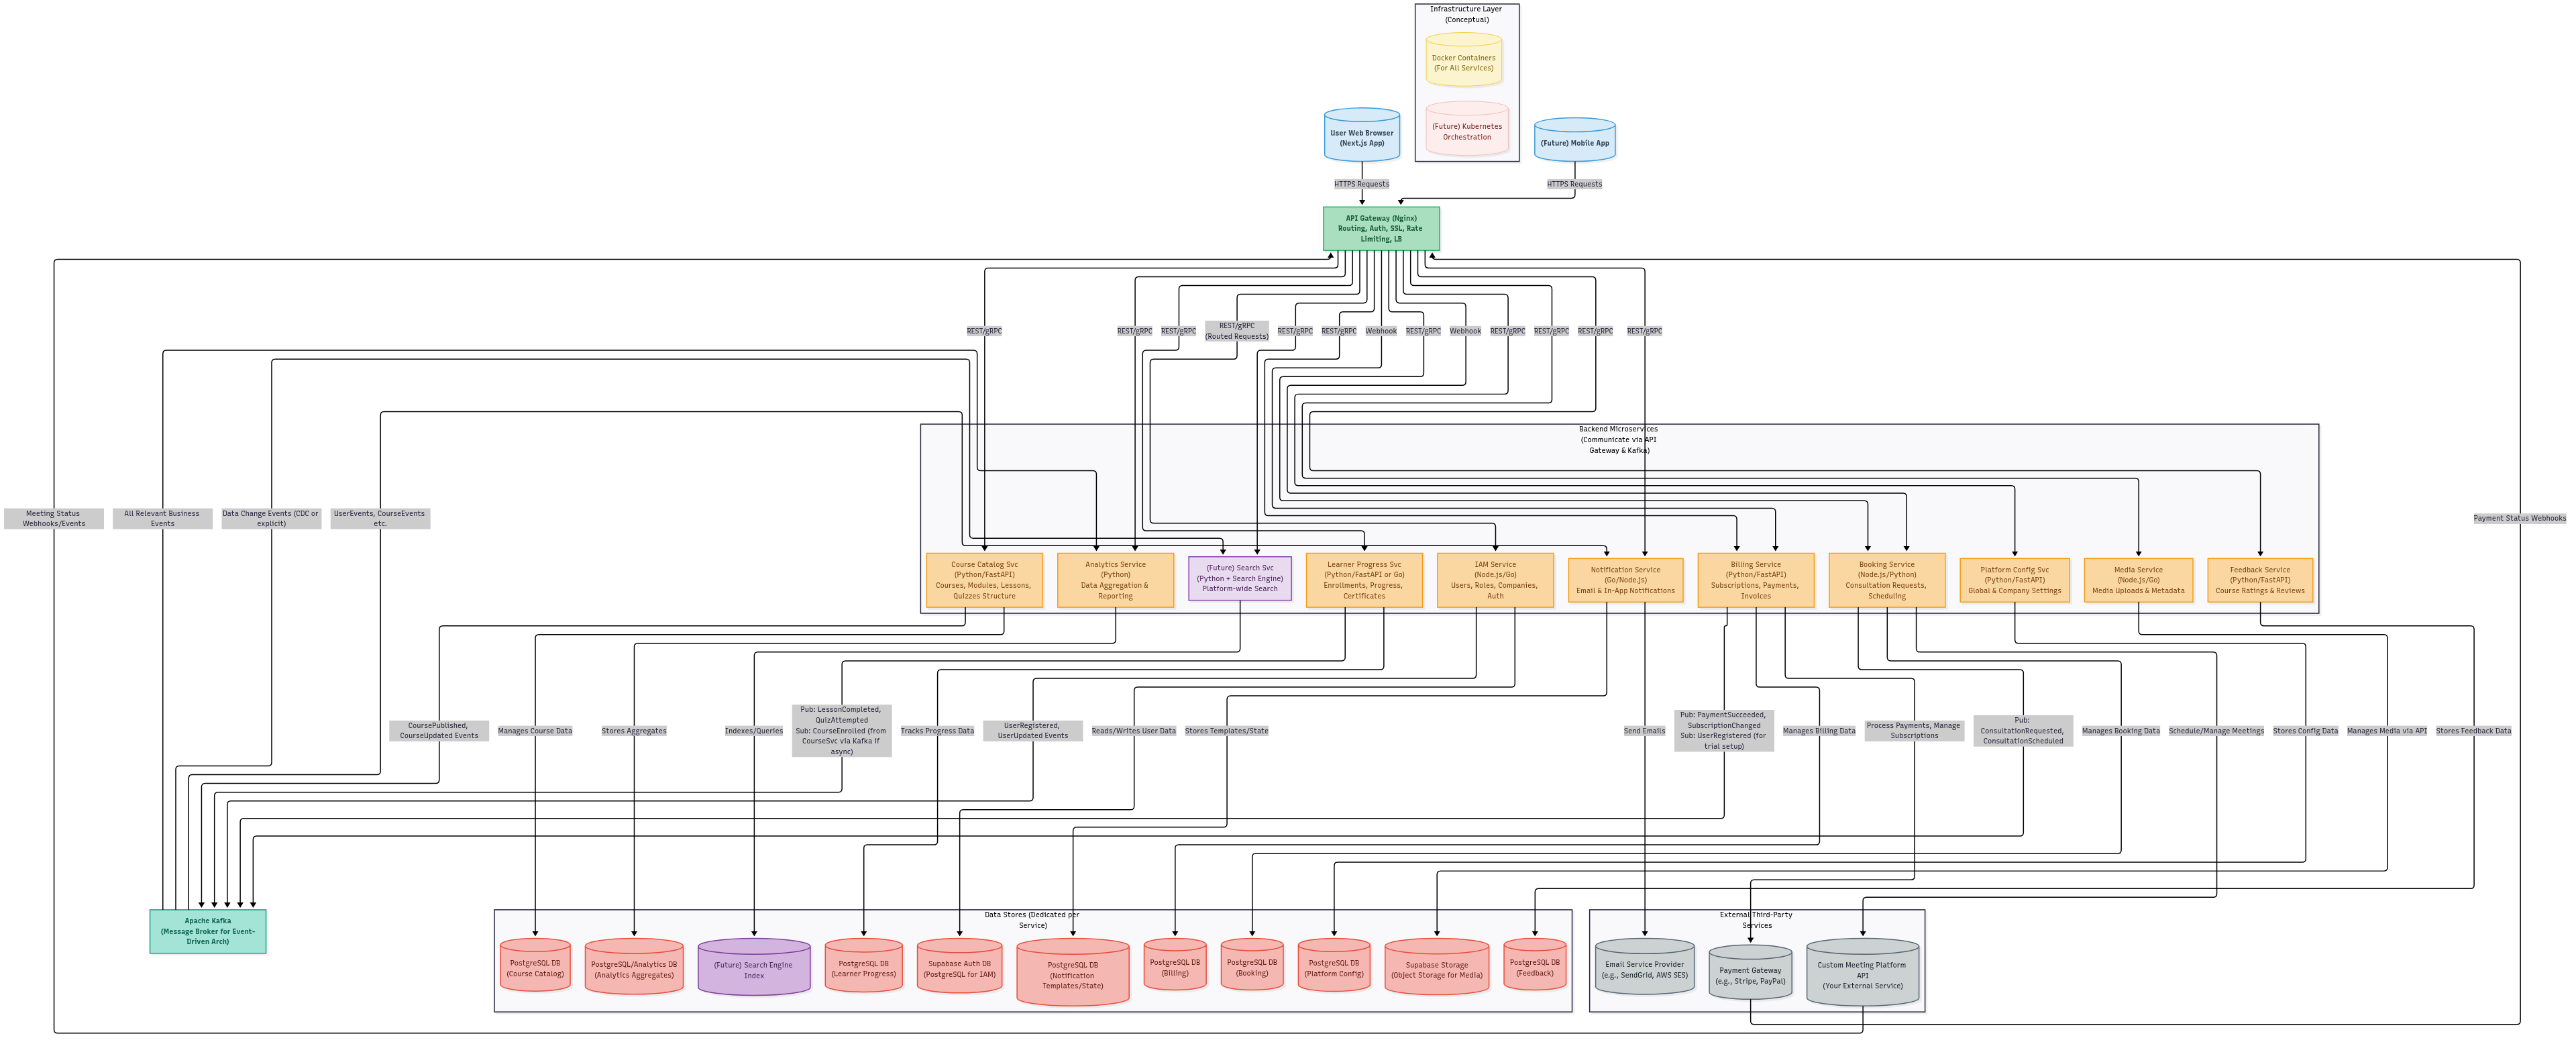
\includegraphics[width=0.9\textwidth,keepaspectratio]{archetecture_diagrame.png}
  \caption{\textbf{Diagramme d'architecture backend} et base de données.}
  \label{fig:architecture_diagram}
\end{figure}

\subsubsection{Exemple de Communication Inter-Services}
\textbf{Scénario : Nouvel utilisateur s'inscrit et s'abonne}
\begin{enumerate}
  \item \textbf{Client (Next.js)} $\rightarrow$ \textbf{Passerelle API (Nginx)} $\rightarrow$ \textbf{Service IAM} (Création de l'utilisateur)
  \item \textbf{Service IAM} $\rightarrow$ \textbf{Kafka} (Publie `UserRegisteredEvent`)
  \item \textbf{Service de Notification} (Consomme l'événement) $\rightarrow$ Envoie un Email de Bienvenue
  \item \textbf{Client} $\rightarrow$ \textbf{Passerelle API} $\rightarrow$ \textbf{Service de Facturation} (Demande d'abonnement)
  \item \textbf{Service de Facturation} $\rightarrow$ Passerelle de Paiement et Mise à jour de la BD interne
  \item \textbf{Service de Facturation} $\rightarrow$ \textbf{Kafka} (Publie `SubscriptionActivatedEvent`)
  \item \textbf{Service IAM} (Consomme, met à jour le statut utilisateur) \& \textbf{Service de Notification} (Consomme, envoie une confirmation)
\end{enumerate}
\textit{Ceci illustre un mélange d'appels API synchrones et de flux événementiels asynchrones.}

% --- Goals for Next Week ---
\section{Objectifs pour la Semaine 2}
\begin{itemize}
  \item \textbf{Familiarisation avec la pile technologique et le projet :} Approfondissement de la compréhension des technologies sélectionnées (Next.js, Go, Python/FastAPI, Node.js, Supabase, Kafka, Docker) et des spécificités du projet
  \item \textbf{Conception de l'expérience utilisateur (UX Design) :} Débuter la création des maquettes (wireframes) et des prototypes pour les interfaces utilisateur clés de la plateforme, en se concentrant sur l'intuitivité et l'efficacité du parcours utilisateur
  \item Affiner les limites des microservices et les contrats d'API
  \item Détailler les schémas de base de données pour chaque service
  \item Planifier les premiers sprints de développement pour les services principaux (par exemple, IAM, Catalogue de Cours)
\end{itemize}

% --- Optional: Conclusion ---
\section{Conclusion Préliminaire}
La première semaine a permis d'établir une fondation solide pour le projet de plateforme e-learning, avec une vision claire, une architecture définie et des acteurs identifiés. Les prochaines étapes se concentreront sur la concrétisation technique et la conception de l'expérience utilisateur.

\end{document}